\mysubsectionformatted{Design Pattern Template}
\myparagraph{

    \begin{tcolorbox}[colback=blue!5!white, colframe=blue!75!black]
        Definisce lo scheletro in un'operazione, lasciando alle sottoclassi di \\modificare
        l'algoritmo senza cambiare la sua struttura.
    \end{tcolorbox}
    \noindent Usiamo \textit{Template} quando si vuole implementare le invarianti di un algoritmo una sola volta,
    saranno le sottoclassi a implementare le varie varianti.

    \subsubsection{Struttura del pattern Template}
    \begin{center}
        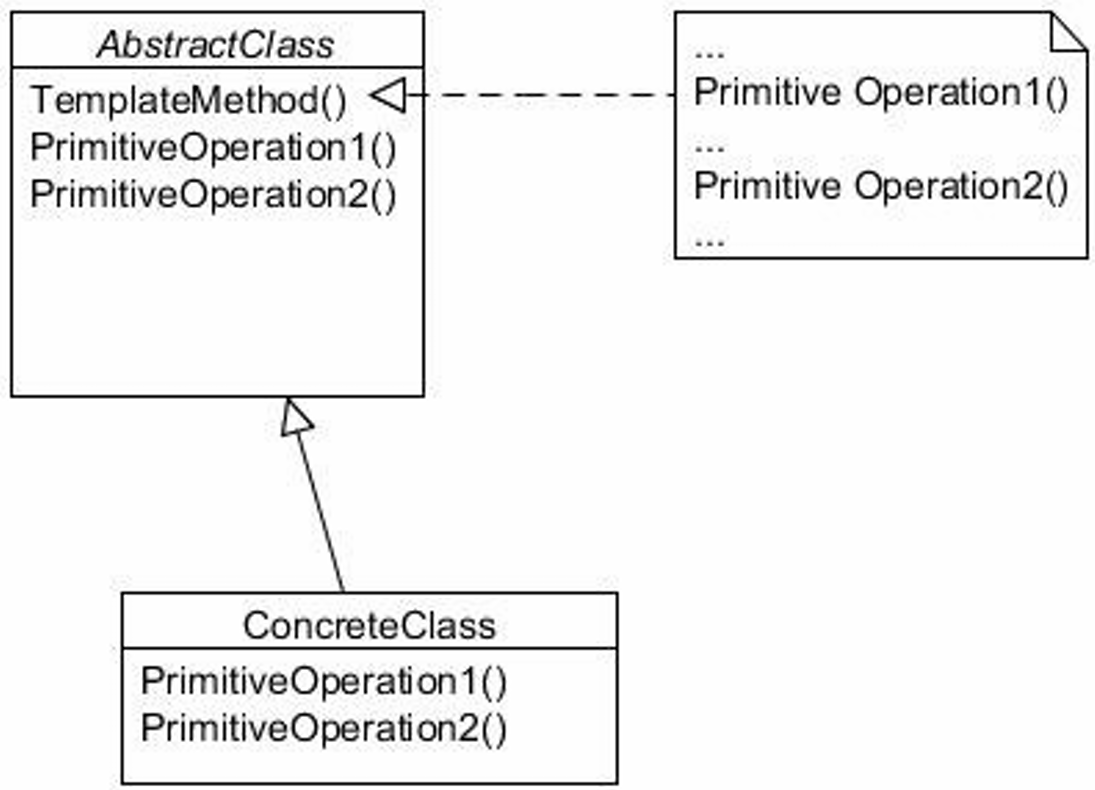
\includegraphics[scale=0.25]{Esercitazione - Design Patterns/template_pattern.png}
    \end{center}
    \begin{enumerate}
        \item \textit{\textbf{AbstractClass}} è la classe che definisce le operazioni primitive di tipo astratto.
        Queste vengono poi implementate dalle sottoclassi \textbf{ConcreteClass}. Definisce un metodo \textbf{TemplateMethod()}
        che rappresenta lo scheletro di un algoritmo e richiama le operazioni primitive.
        \item \textbf{ConcreteClass} sono le classi che implementano le operazioni primitive per poterne variare il 
        comportamento.
    \end{enumerate}
    I metodi template sono fondamentali per il riutilizzo del codice, soprattutto nelle librerie di classi, questo perchè
    sono i mezzi per estrapolare i comportamenti comuni in classi di libreria. Bisogna sempre specificare quali operazione 
    si vogliono sovrascrivere e quali metodi trasferiti alle sottoclassi.

    \newpage
    \subsubsection{Esempio di Design Pattern Template}
    \begin{center}
        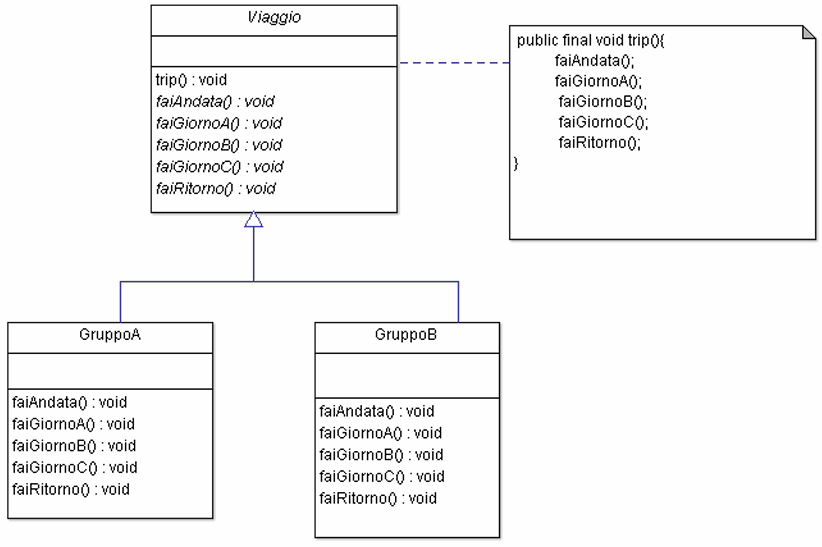
\includegraphics[scale=0.5]{Esercitazione - Design Patterns/example_template_pattern.png}
    \end{center}
    In questo esempio, \textit{Viaggio} è l'\textit{\textbf{AbstractClass}} che contiene il metodo Template \textbf{trip()}. Le
    \textbf{ConcreteClass} \textbf{GruppoA} e \textbf{GruppoB} ereditano i metodi dalla superclasse, decidendo però come deve essere
    implementato ciascun metodo.

    \newpage
}